\documentclass[10pt]{article}
\usepackage{graphicx}
\usepackage[margin=0.8in]{geometry}
\usepackage[T1]{fontenc}
\usepackage{amsmath}
\usepackage{booktabs}
\usepackage{float}
\usepackage{enumitem}
\usepackage{hyperref}
\usepackage{pdfpages}

\setlist{itemsep=2pt, topsep=3pt}
\setlength{\textfloatsep}{8pt plus 2pt minus 2pt}
\setlength{\floatsep}{8pt plus 2pt minus 2pt}
\setlength{\intextsep}{8pt plus 2pt minus 2pt}
\setlength{\abovecaptionskip}{4pt}

\begin{document}

\begin{center}
{\Large Transformer Blocks $|$ Dissecting a Pretrained LLM}\\[6pt]
CSE 256 PA2 \quad$\cdot$\quad Thanh Trinh \quad$\cdot$\quad TSS: 200197841 \quad$\cdot$\quad November 13, 2026
\end{center}

\noindent\textbf{Part A} covers Parts 1 and 2 (encoder and decoder trained from scratch). \textbf{Part B}, attached
after this report, is the PDF export of my executed Part 3 notebook (\texttt{part3.ipynb}).

\section{Part 1: Encoder Trained with a Classifier}

\subsection{Implementation}

Everything is implemented from scratch in \texttt{transformer.py} using only \texttt{nn.Linear},
\texttt{nn.Embedding} and \texttt{nn.LayerNorm}. Each attention head projects its input to queries, keys and values
of size $n_\text{embd}/n_\text{head} = 32$, computes $\mathrm{softmax}(QK^\top/\sqrt{32})V$ and returns its attention
matrix. Multi-head attention concatenates the two heads and applies an output projection. A Transformer block is
pre-LayerNorm: $x \leftarrow x + \mathrm{MHA}(\mathrm{LN}(x))$, then $x \leftarrow x + \mathrm{FFN}(\mathrm{LN}(x))$,
where the feedforward network is Linear(64, 100) $\to$ ReLU $\to$ Linear(100, 64). Token and learned absolute
position embeddings are added before the first of the 4 blocks, and a final LayerNorm follows the last.

Segments are padded to 32 tokens with \texttt{<pad>} (id 0), so the encoder masks padding positions out of every
attention row, and the classifier averages the encoder's output vectors over the \emph{real} tokens only. Without
these masks, a short segment's representation would be dominated by padding. The classifier is a feedforward network
with one hidden layer, Linear(64, 100) $\to$ ReLU $\to$ Linear(100, 3). Encoder and classifier are trained jointly
from scratch with cross-entropy and Adam (lr $10^{-3}$, batch size 16, 15 epochs), all hyperparameters from
\texttt{main.py}.

\textbf{Parameters.} The encoder has \textbf{481,424} parameters: 360,576 in the token embedding (5,634 words
$\times$ 64), 2,048 in the position embedding, 29,668 per block (attention 16,448, feedforward 12,964, two
LayerNorms 256) and 128 in the final LayerNorm. The classifier adds 6,803, for 488,227 in total.

\subsection{Results}

Table~\ref{tab:cls} and Figure~\ref{fig:cls} show accuracy after every epoch. The final test accuracy is
\textbf{85.33\%}, in the expected low to mid 80s; the best epoch reaches 86.40\% (epoch 11). The three speakers are
balanced in \texttt{test\_CLS.tsv} (250 segments each), so chance is 33.3\%.

\begin{table}[htbp]
\centering
\setlength{\tabcolsep}{4pt}
\resizebox{\linewidth}{!}{%
\begin{tabular}{lccccccccccccccc}
\toprule
Epoch & 1 & 2 & 3 & 4 & 5 & 6 & 7 & 8 & 9 & 10 & 11 & 12 & 13 & 14 & 15 \\
\midrule
Train acc. (\%) & 46.6 & 56.4 & 67.2 & 77.0 & 84.9 & 90.3 & 95.5 & 96.6 & 98.1 & 98.2 & 99.2 & 98.8 & 99.8 & 98.2 & 99.4 \\
Test acc. (\%) & 42.7 & 49.6 & 65.7 & 68.7 & 75.6 & 79.5 & 83.7 & 84.1 & 84.5 & 85.3 & 86.4 & 85.5 & 86.3 & 84.5 & \textbf{85.3} \\
\bottomrule
\end{tabular}}
\caption{Part 1 train and test accuracy after each epoch (seed 42).}
\label{tab:cls}
\end{table}

\begin{figure}[htbp]
\centering
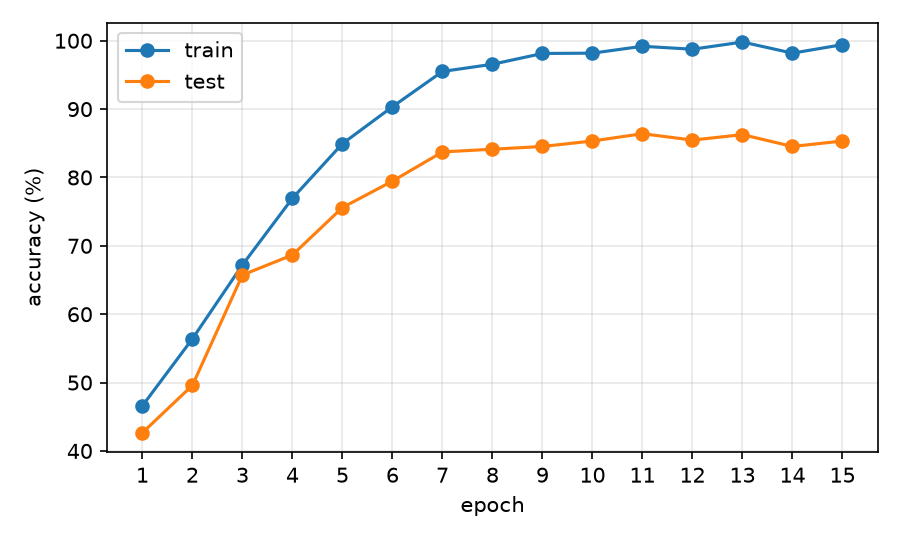
\includegraphics[width=0.6\linewidth]{figures/part1_accuracy.png}
\caption{Part 1 accuracy per epoch.}
\label{fig:cls}
\end{figure}

Test accuracy rises quickly until epoch 7 (83.7\%) and then plateaus around 84--86\%, while training accuracy keeps
climbing to over 99\%. With only 2,092 training segments and about 480k parameters (three quarters of them in the
embedding table), the model starts memorizing after epoch 7, but test accuracy does not collapse.

\subsection{Sanity Checks and Attention Maps}

The provided \texttt{utilities.py} sanity check passes for both test sentences: the largest deviation of any
attention row sum from 1, over all 8 maps (4 layers $\times$ 2 heads), is $2.4 \times 10^{-7}$.
Figure~\ref{fig:enc-attn} shows all 8 maps for \emph{``We must never give up, and we will never give in.''}

\begin{figure}[htbp]
\centering
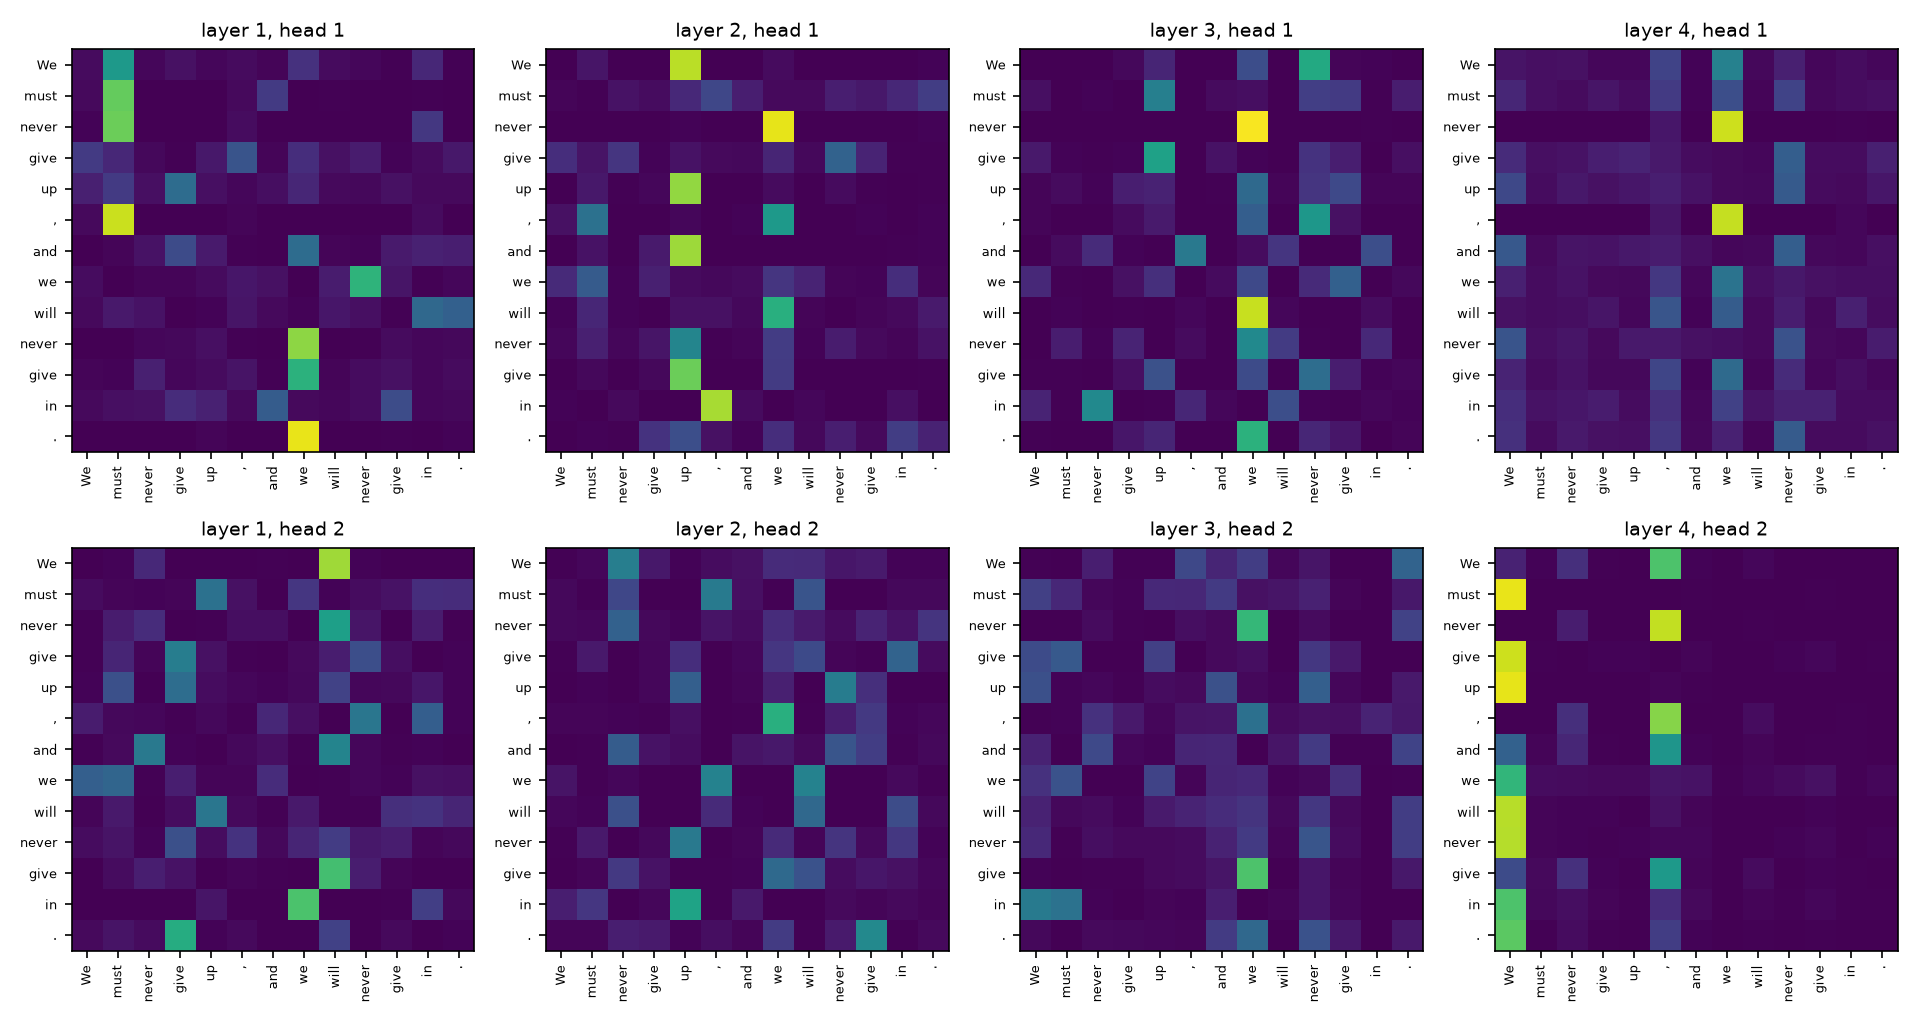
\includegraphics[width=\linewidth]{figures/encoder_attention_s1.png}
\caption{Encoder attention for ``We must never give up, and we will never give in.'' Rows are queries, columns are
keys; every row sums to 1.}
\label{fig:enc-attn}
\end{figure}

\begin{itemize}
  \item \textbf{No mask, so attention goes both ways.} Words attend to words after them as well as before (for
        example in layer 2, head 1, ``We'' attends mostly to ``up'', later in the sentence).
  \item \textbf{Attention concentrates in vertical stripes.} Most heads send many queries to the same one or two
        keys rather than to nearby words: layer 1, head 1 points many rows at ``must''; layer 3, head 1 at ``never''
        and ``we''; layer 4, head 2 sends almost every row to the first word ``We''. Since the classifier only sees
        the average of the outputs, the encoder benefits from collecting information from a few informative words
        into every position.
  \item \textbf{Clauses are linked through their subject.} In layer 1, head 1 the second ``never'', the second
        ``give'' and the final period all attend to ``we'', the subject of the second clause.
\end{itemize}

\section{Part 2: Pretraining a Decoder Language Model}

\subsection{Implementation}

The decoder reuses the same blocks (feedforward hidden size 100 with ReLU) with a causal mask: before the softmax,
every score with key index $j >$ query index $i$ is set to $-\infty$, so each position sees only itself and the
past. After the final LayerNorm, a linear layer maps to the 5,634-word vocabulary, and the loss is the cross-entropy
of the next word at every position. Training uses the base settings: 500 iterations of Adam (lr $10^{-3}$) with
batch size 16 and block size 32, about 256,000 tokens. Following the starter's \texttt{compute\_perplexity}
(\texttt{eval\_iters} = 200), perplexity is $\exp$ of the mean loss over the first 200 batches of 32-token windows,
which covers 58\% (Obama) to 67\% (both Bushes) of each test set; I also report the final perplexity over the full
test sets.

I fixed one bug in the starter \texttt{compute\_perplexity}: it added to an undefined \texttt{total\_loss}. It now
also runs under \texttt{torch.no\_grad()}.

\textbf{Parameters.} The decoder has \textbf{847,634} parameters: the same 481,424 as the encoder (embeddings,
4 blocks, final LayerNorm) plus 366,210 in the output layer ($64 \times 5{,}634$ weights and 5,634 biases).

\subsection{Results}

\begin{table}[htbp]
\centering
\small
\begin{tabular}{lccccc}
\toprule
Iteration & 100 & 200 & 300 & 400 & 500 (final) \\
\midrule
Train & 576.4 & 430.7 & 309.2 & 223.9 & \textbf{171.8} \\
Obama (\texttt{test\_LM\_obama.txt}) & 695.9 & 576.5 & 477.0 & 415.0 & \textbf{384.2} \\
W.\ Bush (\texttt{test\_LM\_wbush.txt}) & 796.5 & 658.1 & 563.7 & 507.8 & \textbf{485.6} \\
H.\ W.\ Bush (\texttt{test\_LM\_hbush.txt}) & 704.6 & 572.9 & 477.2 & 420.7 & \textbf{395.4} \\
\bottomrule
\end{tabular}
\caption{Part 2 perplexity every 100 iterations (seed 42).}
\label{tab:ppl}
\end{table}

\begin{figure}[htbp]
\centering
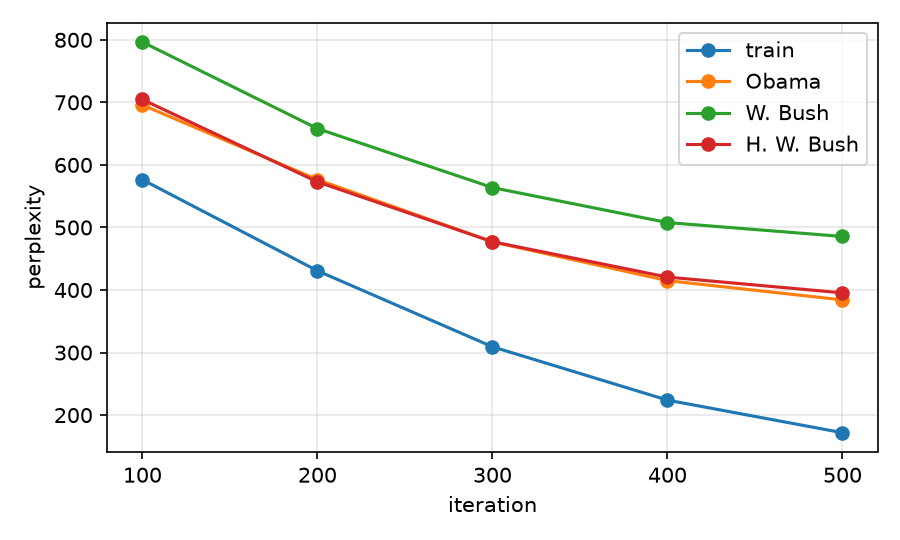
\includegraphics[width=0.6\linewidth]{figures/part2_perplexity.png}
\caption{Part 2 train and test perplexity during pretraining.}
\label{fig:ppl}
\end{figure}

The final training perplexity is \textbf{171.8} (expected: high 100s), and the test perplexities are
\textbf{384.2} (Obama), \textbf{395.4} (H.\ W.\ Bush) and \textbf{485.6} (W.\ Bush), in the expected 300s and 400s
(Table~\ref{tab:ppl}, Figure~\ref{fig:ppl}). Over the full test sets the final perplexities are 374.3 (Obama),
400.5 (H.\ W.\ Bush) and 501.2 (W.\ Bush), with the same ranking. All curves are still falling at iteration 500, but the gap between train
and test widens: \texttt{train\_LM.txt} has only 32,288 tokens, so 256,000 training tokens cover it about 8 times.

\textbf{Why the politicians get different perplexities.} I measured two properties of the data that line up with
the ranking Obama $<$ H.\ W.\ Bush $<$ W.\ Bush:
\begin{itemize}
  \item \textbf{How much of each speaker the model saw.} \texttt{train\_LM.txt} is unlabeled, but the labeled
        \texttt{train\_CLS.tsv}, drawn from the same speeches, is 45\% Obama (934 segments), 30\% H.\ W.\ Bush (619)
        and 26\% W.\ Bush (539). If the language-modeling text has a similar mix, the decoder has learned Obama's
        phrasing, topics and favourite words best, and W.\ Bush's least.
  \item \textbf{How many test words are rare in training.} The share of unknown words is almost the same for all
        three (1.9\% Obama, 2.1\% for both Bushes), but the share of test tokens that appear at most twice in
        \texttt{train\_LM.txt} differs: 14.8\% for Obama, 16.6\% for H.\ W.\ Bush and 18.3\% for W.\ Bush. Words
        seen once or twice get poorly estimated probabilities, so W.\ Bush's speeches, which use more vocabulary
        the model barely saw, are hardest to predict.
\end{itemize}
Speaking style matters too: each politician has recurring topics and phrases (for example W.\ Bush's speeches about
terrorism and Iraq), and a test set whose topics are well covered in training is easier.

\subsection{Sanity Checks and Attention Maps}

The sanity check passes again (largest row-sum deviation $1.8 \times 10^{-7}$). Figure~\ref{fig:dec-attn} shows the
decoder's 8 maps for the same sentence.

\begin{figure}[htbp]
\centering
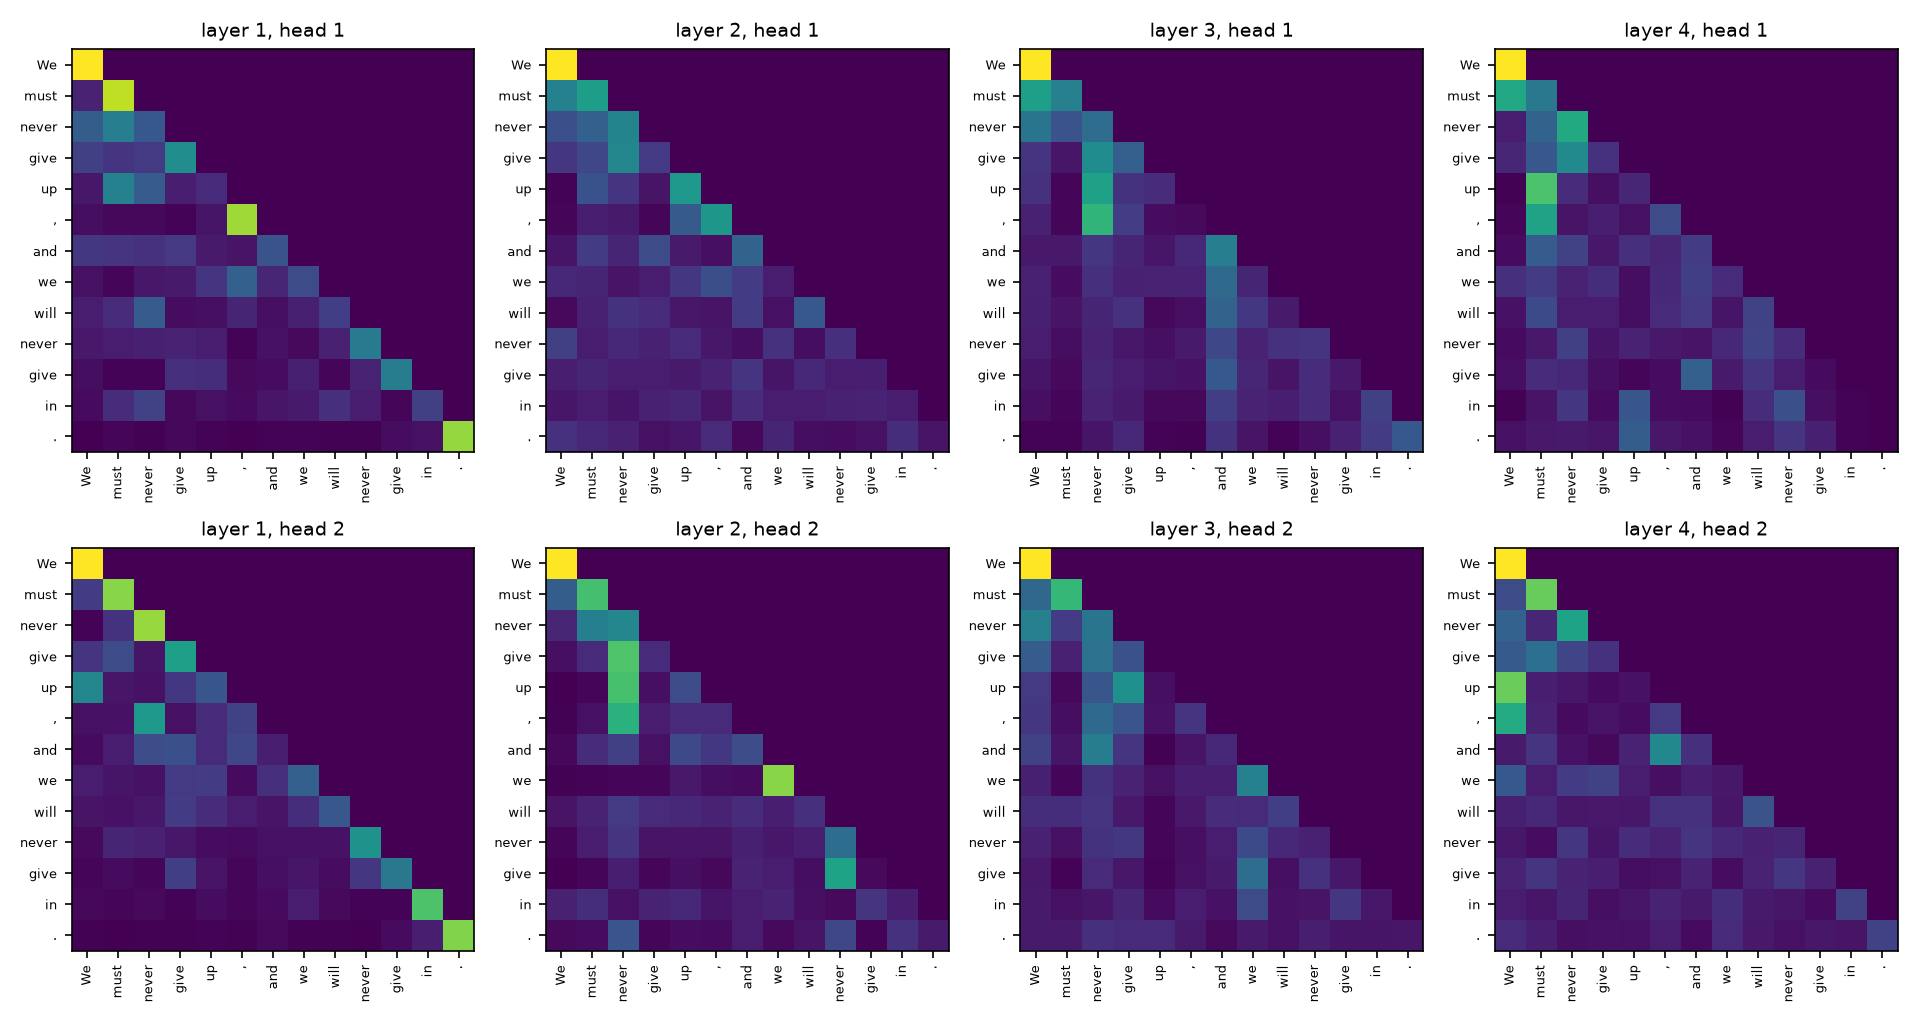
\includegraphics[width=\linewidth]{figures/decoder_attention_s1.png}
\caption{Decoder attention for ``We must never give up, and we will never give in.'' The upper triangle is exactly
zero because of the causal mask.}
\label{fig:dec-attn}
\end{figure}

\begin{itemize}
  \item \textbf{The mask is visible as a lower-triangular pattern.} Every entry above the diagonal is exactly zero,
        so no word attends to the future. The first row always puts weight 1 on ``We'', because it is the only
        visible word, and each row still sums to 1 over the words it can see.
  \item \textbf{Layer 1 looks mostly at the current word.} Both heads in layer 1 have a strong diagonal, so each
        position starts by attending to itself (and sometimes the previous word).
  \item \textbf{Deeper layers spread over the past and reuse anchor words.} In layers 2--4 attention is more
        diffuse, and several heads keep returning to the first word and to ``never'' (a bright column in layer 2,
        head 2), which acts as a summary of the earlier context.
\end{itemize}
Unlike the encoder, which can gather evidence from the whole segment, the decoder can only look back, so its maps
show where the model looks when predicting the next word.

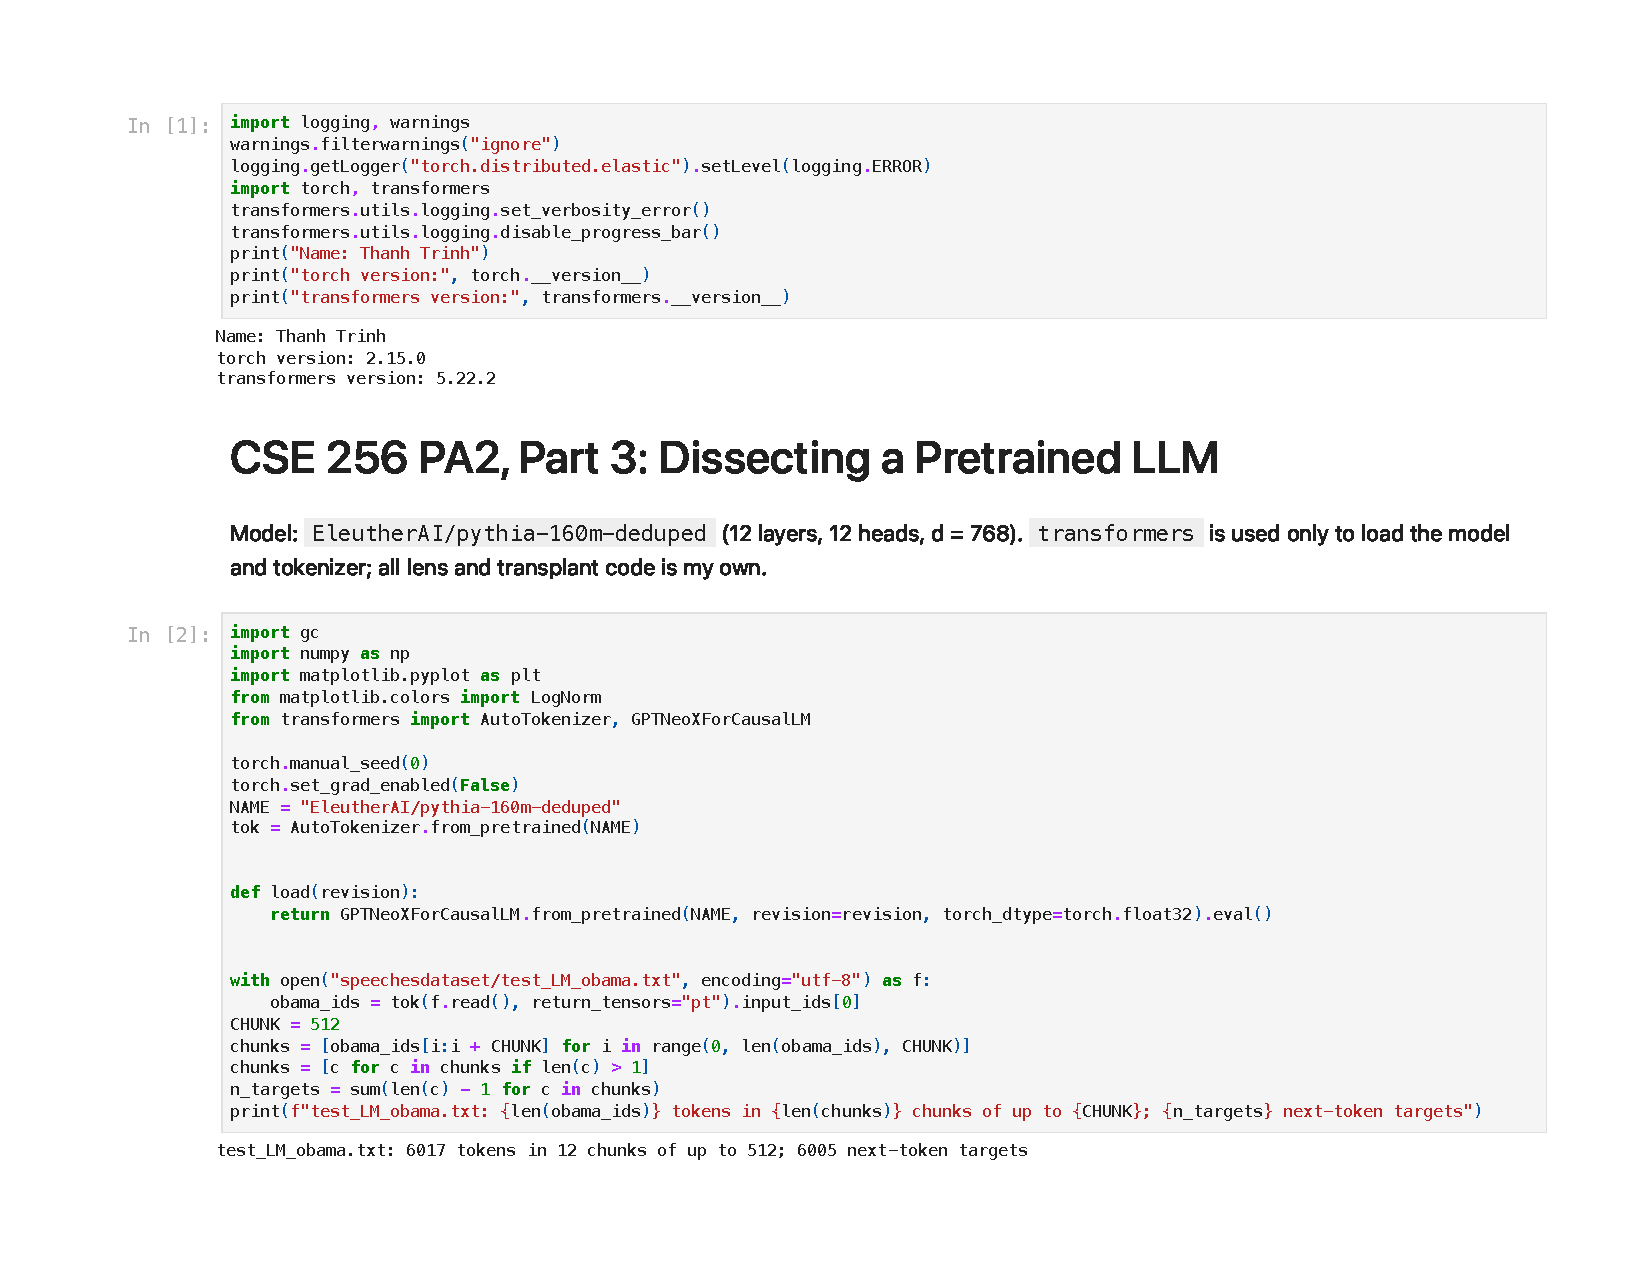
\includepdf[pages=-, fitpaper=true]{part3_notebook.pdf}

\end{document}
